\begin{figure}[t]
    \centering
    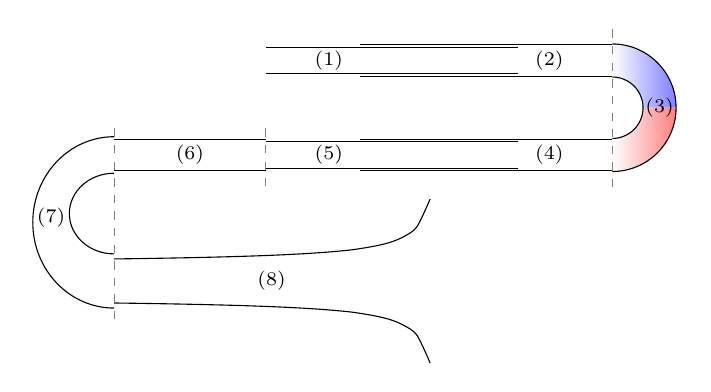
\begin{tikzpicture}[scale = 8]

    \def\labelColor{black};
    \def\labelSize{\fontsize{7pt}{7pt}\selectfont};

    \def\hornOffset{0.025};
    \def\stepSize{0.004}

    \def\dashedLineColor{gray};
    \def\dashedLineOvershoot{0.025}
    % tuning slide params
    \def\tuningSlideDim{0.1};
    \pgfmathsetmacro{\tuningSlideRad}{\stepSize + \hornOffset};
    \def\tuningSlideOffset{0.007};

    % gooseneck params
    \def\gooseNeckLength{0.241};
    \pgfmathsetmacro{\gooseNeckRad}{\tuningSlideRad - \stepSize};

    % inner slide params
    \def\innerLength{0.4};
    \pgfmathsetmacro{\innerRad}{\gooseNeckRad - \stepSize};

    % outer slide params
    \def\outerLength{\innerLength};
    \pgfmathsetmacro{\outerRad}{\gooseNeckRad};
    \pgfmathsetmacro{\extension}{0.15};

    \def\endOfSlideDim{0.075};
    \pgfmathsetmacro{\endOfSlideRad}{\outerRad * 1.05};

    %% draw horn

    \draw[domain=0:0.502, smooth, variable=\x, black] plot ({\x}, {\hornOffset + 0.0063 * ((0.502-\x) + 0.0174)^(-0.7)});
    
    \draw[domain=0:0.502, smooth, variable=\x, black] plot ({\x}, {-\hornOffset-0.0063 * ((0.502-\x) + 0.0174)^(-0.7)});
    
    \node[anchor = center, color = \labelColor](eight) at (0.25, 0) {\labelSize(8)};

    % draw tuningSlide
    \pgfmathsetmacro{\innerTuningSlideDim}{(\tuningSlideDim - \tuningSlideRad)}
    \pgfmathsetmacro{\outerTuningSlideDim}{(\tuningSlideDim + \tuningSlideRad)}

    \node[anchor = center, color = \labelColor](seven) at (-\innerTuningSlideDim-\tuningSlideRad, \innerTuningSlideDim+\tuningSlideRad) {\labelSize(7)};

    \pgfmathsetmacro{\innerTuningSlideWithOffset}{\innerTuningSlideDim - \tuningSlideOffset}

    \pgfmathsetmacro{\outerTuningSlideWithOffset}{\outerTuningSlideDim + \tuningSlideOffset}

    \draw (0, 2*\tuningSlideDim-\tuningSlideRad) arc(90:270:\innerTuningSlideDim cm and \innerTuningSlideWithOffset cm);

    \draw (0, 2*\tuningSlideDim+\tuningSlideRad) arc(90:270:\outerTuningSlideDim cm and \outerTuningSlideWithOffset cm);
    
    % dashedline
    \draw[dashed, color = \dashedLineColor] (0, -\tuningSlideRad-\tuningSlideOffset-\dashedLineOvershoot) -- (0, 2*\tuningSlideDim+\tuningSlideRad+\dashedLineOvershoot);

    % draw gooseneck
    \draw (0, 2*\tuningSlideDim + \gooseNeckRad) -- (\gooseNeckLength, 2*\tuningSlideDim + \gooseNeckRad);

    \draw (0, 2*\tuningSlideDim - \gooseNeckRad) -- (\gooseNeckLength, 2*\tuningSlideDim - \gooseNeckRad);

    \node[anchor = center, color = \labelColor](six) at (0.5 * \gooseNeckLength, 2*\tuningSlideDim) {\labelSize(6)};

    % dashedline
    \draw[dashed, color = \dashedLineColor] (\gooseNeckLength, 2*\tuningSlideDim-\gooseNeckRad-\dashedLineOvershoot) -- (\gooseNeckLength, 2*\tuningSlideDim+\gooseNeckRad+\dashedLineOvershoot);

    % draw inner slide
    \draw (\gooseNeckLength, 2*\tuningSlideDim + \innerRad) -- (\gooseNeckLength+\innerLength, 2*\tuningSlideDim + \innerRad);

    \draw (\gooseNeckLength, 2*\tuningSlideDim - \innerRad) -- (\gooseNeckLength+\innerLength, 2*\tuningSlideDim - \innerRad);

    \node[anchor = center, color = \labelColor](five) at (\gooseNeckLength + 0.25 * \innerLength, 2*\tuningSlideDim) {\labelSize(5)};

    % draw outer slide
    \pgfmathsetmacro{\outerSlideStart}{\gooseNeckLength + \extension};

    \draw (\outerSlideStart, 2*\tuningSlideDim + \outerRad) -- (\outerSlideStart+\outerLength, 2*\tuningSlideDim + \outerRad);

    \draw (\outerSlideStart, 2*\tuningSlideDim - \outerRad) -- (\outerSlideStart+\outerLength, 2*\tuningSlideDim - \outerRad);

    \node[anchor = center, color = \labelColor](four) at (\outerSlideStart + 0.75 * \outerLength, 2*\tuningSlideDim) {\labelSize(4)};


    % draw end of slide
    
    \pgfmathsetmacro{\innerEndOfSlideDim}{(\endOfSlideDim - \endOfSlideRad)};
    \pgfmathsetmacro{\outerEndOfSlideDim}{(\endOfSlideDim + \endOfSlideRad)};

    \pgfmathsetmacro{\startEndOfSlide}{\outerSlideStart + \outerLength};
    % division blue
    \fill[white, left color=white, right color=blue, fill opacity = 0.5] 
    (\startEndOfSlide+\innerEndOfSlideDim,2*\tuningSlideDim+\endOfSlideDim) 
    arc (0:90:\innerEndOfSlideDim cm and \innerEndOfSlideDim cm) 
    -- (\startEndOfSlide,2*\tuningSlideDim+\endOfSlideDim + \innerEndOfSlideDim)
    -- (\startEndOfSlide,2*\tuningSlideDim+2*\endOfSlideDim+\endOfSlideRad)
    arc (90:0:\outerEndOfSlideDim cm and \outerEndOfSlideDim cm)
    -- (\startEndOfSlide+\outerEndOfSlideDim,2*\tuningSlideDim+\endOfSlideDim)
    -- cycle;

    % division red
    \fill[white, left color=white, right color=red, fill opacity = 0.5] 
    (\startEndOfSlide+\innerEndOfSlideDim,2*\tuningSlideDim+\endOfSlideDim) 
    arc (0:-90:\innerEndOfSlideDim cm and \innerEndOfSlideDim cm) 
    -- (\startEndOfSlide,2*\tuningSlideDim+\endOfSlideDim)
    -- (\startEndOfSlide,2*\tuningSlideDim-\endOfSlideRad)
    arc (-90:0:\outerEndOfSlideDim cm and \outerEndOfSlideDim cm)
    -- (\startEndOfSlide+\outerEndOfSlideDim,2*\tuningSlideDim+\endOfSlideDim)
    -- cycle;

    \draw (\startEndOfSlide, 2*\tuningSlideDim+\endOfSlideRad) arc(-90:90:\innerEndOfSlideDim cm and \innerEndOfSlideDim cm);

    \draw (\startEndOfSlide, 2*\tuningSlideDim-\endOfSlideRad) arc(-90:90:\outerEndOfSlideDim cm and \outerEndOfSlideDim cm);

    \node[anchor = center, color = \labelColor](three) at (\startEndOfSlide + \innerEndOfSlideDim + \endOfSlideRad, 2*\tuningSlideDim+ \innerEndOfSlideDim + \endOfSlideRad) {\labelSize(3)};


    % dashedline
    \draw[dashed, color = \dashedLineColor] (\startEndOfSlide, 2*\tuningSlideDim-\endOfSlideRad-\dashedLineOvershoot) -- (\startEndOfSlide, 2*\tuningSlideDim+2*\endOfSlideDim+\endOfSlideRad+\dashedLineOvershoot);

    % draw second outer slide

    \draw (\outerSlideStart, 2*\tuningSlideDim + 2 * \endOfSlideDim + \outerRad) -- (\outerSlideStart+\outerLength, 2*\tuningSlideDim + 2 * \endOfSlideDim + \outerRad);

    \draw (\outerSlideStart, 2*\tuningSlideDim + 2 * \endOfSlideDim - \outerRad) -- (\outerSlideStart+\outerLength, 2*\tuningSlideDim + 2 * \endOfSlideDim - \outerRad);

    \node[anchor = center, color = \labelColor](two) at (\outerSlideStart + 0.75 * \outerLength, 2*\tuningSlideDim + 2 * \endOfSlideDim) {\labelSize(2)};

    % draw inner slide
    \draw (\gooseNeckLength, 2*\tuningSlideDim+ 2 * \endOfSlideDim + \innerRad) -- (\gooseNeckLength+\innerLength, 2*\tuningSlideDim+ 2 * \endOfSlideDim + \innerRad);

    \draw (\gooseNeckLength, 2*\tuningSlideDim + 2 * \endOfSlideDim - \innerRad) -- (\gooseNeckLength+\innerLength, 2*\tuningSlideDim + 2 * \endOfSlideDim - \innerRad);

    \node[anchor = center, color = \labelColor](one) at (\gooseNeckLength + 0.25 * \innerLength, 2*\tuningSlideDim + 2 * \endOfSlideDim) {\labelSize(1)};

% \begin{scope}[very thick,decoration={
%     markings,
%     mark=at position 0.5 with {\arrow{>}}}
%     ] 
%     \draw[postaction={decorate}] (-4,0)--(4,0);
% \end{scope}
    
    \end{tikzpicture}
    \caption{\it Diagram showing the trombone geometry (not to scale). Numbers correspond to the parts of the tube found in Table \ref{tab:geometry} and dashed lines highlight where the different parts are separated. The tube is split in the middle of the slide crook with the colours corresponding to those in Figure \ref{fig:dynamicGridSchematic}.}
    \label{fig:tromboneSchematic}
\end{figure}